\section{Installation}

Exists several ways to install own Chef Server:

\begin{itemize}
  \item Go to \href{http://www.getchef.com/chef/install/}{www.getchef.com/chef/install}, select the operating system, version, and architecture of the server and install the downloaded package on it. After installation you can configure server by command <<sudo chef-server-ctl reconfigure>>
  \item Use Chef Solo to install Chef Server
\end{itemize}

Of course, I prefer to use Chef Solo to install and configure Chef Server. Chef Solo will help us quickly deploy Chef Server on a new server, if with it something happens (crash file system of server, etc.). Do not forget to make a backups of Chef Server (because compared with Chef Solo, Chef Server will be the point of failure in your configuration management system).

Let's create our folder, which will contain all our Chef kitchen:

\begin{lstlisting}[language=Bash,label=lst:my-server-cloud-installation1]
$ mkdir my-server-cloud
$ cd my-server-cloud
$ cat Gemfile
source "https://rubygems.org"

gem 'knife-solo'
gem 'berkshelf'
$ bundle
$ knife solo init .
WARNING: No knife configuration file found
Creating kitchen...
Creating knife.rb in kitchen...
Creating cupboards...
Setting up Berkshelf...
\end{lstlisting}

To install and configure Chef Server exists cookbook \href{http://community.opscode.com/cookbooks/chef-server}{chef-server}. Let's add this cookbook in Berkshelf:

\begin{lstlisting}[label=lst:my-server-cloud-installation2,title=my-server-cloud/Berkshelf]
site :opscode

cookbook 'chef-server'
\end{lstlisting}

After running the command <<berks install>> this cookbook will be installed with dependencies.

\begin{lstlisting}[language=Bash,label=lst:my-server-cloud-installation3]
$ berks install
Installing chef-server (2.0.1) from site: 'http://cookbooks.opscode.com/api/v1/cookbooks'
$ berks install --path cookbooks
Using chef-server (2.0.1)
\end{lstlisting}

Now we should configure a Chef Solo node for our Chef Server. From chapter~\ref{sec:solo-node} you should know how to define node.

\begin{lstlisting}[language=JSON,label=lst:my-server-cloud-installation4,title=my-server-cloud/nodes/chef-server.example.com.json]
{
  "fqdn": "10.33.33.33",
  "chef-server": {
    "api_fqdn": "10.33.33.33",
    "version": "latest",
    "configuration": {
      "notification_email": "notify@example.com",
      "chef-server-webui": {
        "enable": true
      }
    }
  },
  "run_list": [
    "recipe[chef-server]"
  ]
}
\end{lstlisting}

By \inline{configuration} key you can change settings for Chef Server. All available setting, which is possible to redefined, you can find \href{https://github.com/opscode/omnibus-chef-server/blob/master/files/chef-server-cookbooks/chef-server/attributes/default.rb}{here}. Our Chef Server by default takes your systems \href{http://en.wikipedia.org/wiki/Fully\_qualified\_domain\_name}{FQDN} as Chef Server url, what is why I set <<fqdn>> in node IP 10.33.33.33, which will set to my server by Vagrant.

First, we should generate Vagrantfile:

\begin{lstlisting}[language=Bash,label=lst:my-server-cloud-installation5]
$ vagrant init precise64
A `Vagrantfile` has been placed in this directory. You are now
ready to `vagrant up` your first virtual environment! Please read
the comments in the Vagrantfile as well as documentation on
`vagrantup.com` for more information on using Vagrant.
\end{lstlisting}

Next we need modeling a cluster of machines by Vagrant. Right now we need only chef server. Let's modify Vagrantfile:

\begin{lstlisting}[label=lst:my-server-cloud-installation6,title=my-server-cloud/Vagrantfile]
# -*- mode: ruby -*-
# vi: set ft=ruby :

require 'chef'
require 'json'

Chef::Config.from_file(File.join(File.dirname(__FILE__), '.chef', 'knife.rb'))

chef_server_json = JSON.parse(Pathname(__FILE__).dirname.join('nodes', 'chef-server.example.com.json').read)

# Vagrantfile API/syntax version. Don't touch unless you know what you're doing!
VAGRANTFILE_API_VERSION = "2"

Vagrant.configure(VAGRANTFILE_API_VERSION) do |config|

  config.vm.define :chef_server do |chef_server|
    chef_server.vm.box = "precise64"
    chef_server.vm.network "private_network", ip: "10.33.33.33"

    chef_server.vm.provision :chef_solo do |chef|
      chef.cookbooks_path = Chef::Config[:cookbook_path]
      chef.roles_path = Chef::Config[:role_path]
      chef.data_bags_path = Chef::Config[:data_bag_path]
      chef.environments_path = Chef::Config[:environment_path]

      chef.run_list = chef_server_json.delete('run_list')
      chef.json = chef_server_json
    end
  end

end
\end{lstlisting}

You should have installed chef gem inside vagrant, as we did in chapter <<\ref{sec:solo-vagrant}~Vagrant>> and install/update Chef Client inside server by command <<knife solo prepare>>.

\begin{lstlisting}[language=Bash,label=lst:my-server-cloud-installation7]
$ vagrant provision
[chef_server] Running provisioner: chef_solo...
Generating chef JSON and uploading...
Running chef-solo...
stdin: is not a tty
[2014-01-05T12:55:12+00:00] INFO: Forking chef instance to converge...
[2014-01-05T12:55:12+00:00] INFO: *** Chef 11.8.2 ***
[2014-01-05T12:55:12+00:00] INFO: Chef-client pid: 1831
[2014-01-05T12:55:13+00:00] INFO: Setting the run_list to ["recipe[chef-server]"] from JSON
[2014-01-05T12:55:13+00:00] INFO: Run List is [recipe[chef-server]]
[2014-01-05T12:55:13+00:00] INFO: Run List expands to [chef-server]
...
\end{lstlisting}

We can check Chef Server web interface by \href{https://10.33.33.33}{https://10.33.33.33} and info about versions by \href{https://10.33.33.33/version}{https://10.33.33.33/version} url. It should looks like on figure~\ref{fig:chef-server-versions}.

\begin{figure}[ht!]
  \center{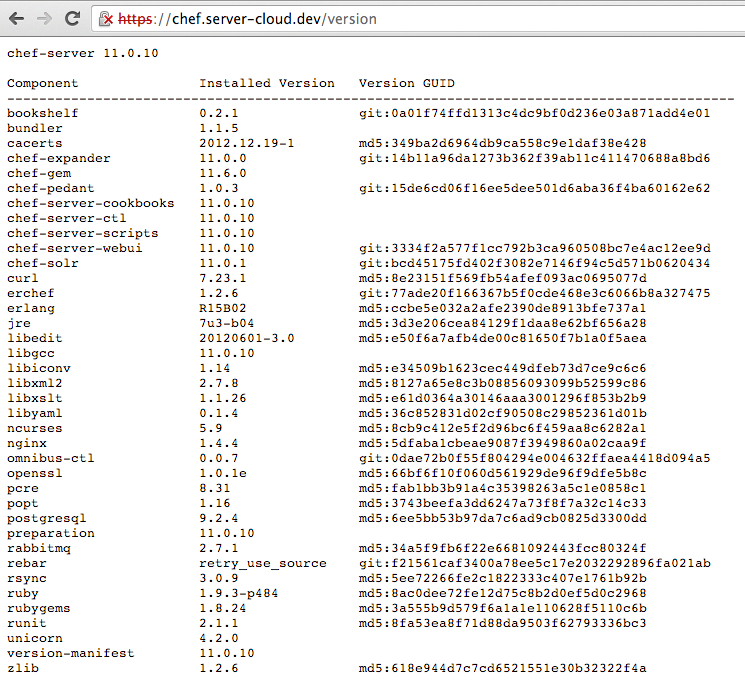
\includegraphics[width=1\textwidth]{chef_server_versions}}
  \caption{Chef Server Versions}
  \label{fig:chef-server-versions}
\end{figure}

I most cases web interface give information about your cloud, which you can get from knife tool. What is why generally it disabled by attribute <<chef-server-webui.enable = false>>.

Next we should configure our knife to work with this Chef Server.
